%%%%%%%%%%%%%%%%%%%%%%%%%%%%%%%%%%%%%%%%%%%%%%%%%%%%%%%%%%%%%%%%%%%%%%%%%%%%%%%%%%%
%% This project aims to create the UNAL template for presentation.               %%
%% author:Félix Julián Gutiérrez                                                 %%
%% contacts:                                                                     %%
%%    e-mail: fjgutierrezb@unal.edu.co                                           %%
%%   www.unal.edu.co                                                             %%
%%%%%%%%%%%%%%%%%%%%%%%%%%%%%%%%%%%%%%%%%%%%%%%%%%%%%%%%%%%%%%%%%%%%%%%%%%%%%%%%%%%
\documentclass{libs/ufc_format}
% Inserting the preamble file with the packages
%%%%%%%%%%%%%%%%%%%%%%%%%%%%%%%%%%%%%%%%%%%%%%%%%%%%%%%%%%%%%%%%%%%%%
%% This file contains the packages that can be used in the beamer. %%
%%%%%%%%%%%%%%%%%%%%%%%%%%%%%%%%%%%%%%%%%%%%%%%%%%%%%%%%%%%%%%%%%%%%%
% Package to fonts family
\usepackage[T1]{fontenc}
% Package to accentuation
\usepackage[utf8]{inputenc}
% Package to Spanish language
\usepackage[spanish]{babel}
% Package to Figures
\usepackage{graphicx}
% Package to the colors
\usepackage{color}
% Package to the colors
\usepackage{xcolor}
% Packages to math symbols and expressions
\usepackage{amsfonts, amssymb, amsmath}
% Package to multiple lines and columns in table
\usepackage{multirow, array} 
% Package to create pseudo-code
% For more detail of this package: http://linorg.usp.br/CTAN/macros/latex/contrib/algorithm2e/doc/algorithm2e.pdf
\usepackage{algorithm2e}
% Package to insert code
\usepackage{listings} 
\usepackage{keyval}
% Package to justify text
\usepackage[document]{ragged2e}
% Package to manage the bibliography
\usepackage[backend=biber, style=numeric, sorting=none]{biblatex}
% Package to facilities quotations
\usepackage{csquotes}
% Package to use multicols
\usepackage{multicol}

% SVG (CUSTOM)
\usepackage{svg}
% Inserting the references file
\bibliography{references.bib}

% Title
\title[Sistemas Operativos]{\huge\textbf{}}
% Subtitle
\subtitle{\textbf{El Sistema Operativo XV6 - Capítulo 2 - Parte 2}}
% Author of the presentation
\author{Carlos Santiago Sandoval Casallas}
% Institute's Name
\institute[UNAL]{
    % email for contact
    \normalsize{\email{csandovalc@unal.edu.co}}
    \newline
    % Department Name
    \department{Departamento de Ingeniería de Sistemas e Industrial}
    \newline
    % university name
    \ufc
}
% date of the presentation
\date{\today}

%%%%%%%%%%%%%%%%%%%%%%%%%%%%%%%%%%%%%%%%%%%%%%%%%%%%%%%%%%%%%%%%%%%%%%%%%%%%%%%%%%
%% Start Document of the Presentation                                           %%               
%%%%%%%%%%%%%%%%%%%%%%%%%%%%%%%%%%%%%%%%%%%%%%%%%%%%%%%%%%%%%%%%%%%%%%%%%%%%%%%%%%
\begin{document}
% insert the code style
%%%%%%%%%%%%%%%%%%%%%%%%%%%%%%%%%%%%%%%%%%%%%%%%%%%%%%%%%%%%%%%%%%%%%%%%%%%%%%%%%%%
%% This file contains the style of the codes show in slides.                     %%
%% The package used is listings, but it possible to used others.                 %%
%%%%%%%%%%%%%%%%%%%%%%%%%%%%%%%%%%%%%%%%%%%%%%%%%%%%%%%%%%%%%%%%%%%%%%%%%%%%%%%%%%%

% color used in the code style
\definecolor{codegreen}{rgb}{0,0.6,0}
\definecolor{codegray}{rgb}{0.5,0.5,0.5}
\definecolor{codepurple}{rgb}{0.58,0,0.82}
\definecolor{codebackground}{rgb}{0.95,0.95,0.92}

% style of the code!
\lstdefinestyle{codestyle}{
    backgroundcolor=\color{codebackground},   
    commentstyle=\color{codegreen},
    keywordstyle=\color{magenta},
    numberstyle=\tiny\color{codegray},
    stringstyle=\color{codepurple},
    basicstyle=\ttfamily\footnotesize,
    frame=single,
    breakatwhitespace=false,         
    breaklines=true,                 
    captionpos=b,                    
    keepspaces=true,                 
    numbers=left,                    
    numbersep=5pt,                  
    showspaces=false,                
    showstringspaces=false,
    showtabs=false,                  
    tabsize=2,
    title=\lstname 
}

\lstset{style=codestyle}


%% ---------------------------------------------------------------------------
% First frame (with tile, subtitle, ...)
\begin{frame}
    \maketitle
\end{frame}

%% ---------------------------------------------------------------------------
% Second frame
\begin{frame}{Agenda}
    % \begin{multicols}{2}
        \tableofcontents
    % \end{multicols}
\end{frame}
%% ---------------------------------------------------------------------------
\section{Organización de XV6}
\begin{frame}{Organización del kernel}
    El código fuente del kernel se encuentra en el subdirectorio \href{https://github.com/CarlosSandoval-03/xv6-riscv/tree/riscv/kernel}{\textit{“kernel”}}, este se divide en archivos, buscando una noción de modularidad \cite{xv6_book}.

    \vspace{0.3cm}

    En la figura \ref{fig:Espacio_Direcciones} se enumeran los archivos y su descripción. Las interfaces entre módulos se definen en \href{https://github.com/CarlosSandoval-03/xv6-riscv/blob/riscv/kernel/defs.h}{\textit{\textbf{kernel/defs.h}}}
\end{frame}
%% ---------------------------------------------------------------------------
\begin{frame}
    \begin{figure}
        \centering
        \caption{Estructura del kernel XV6}
        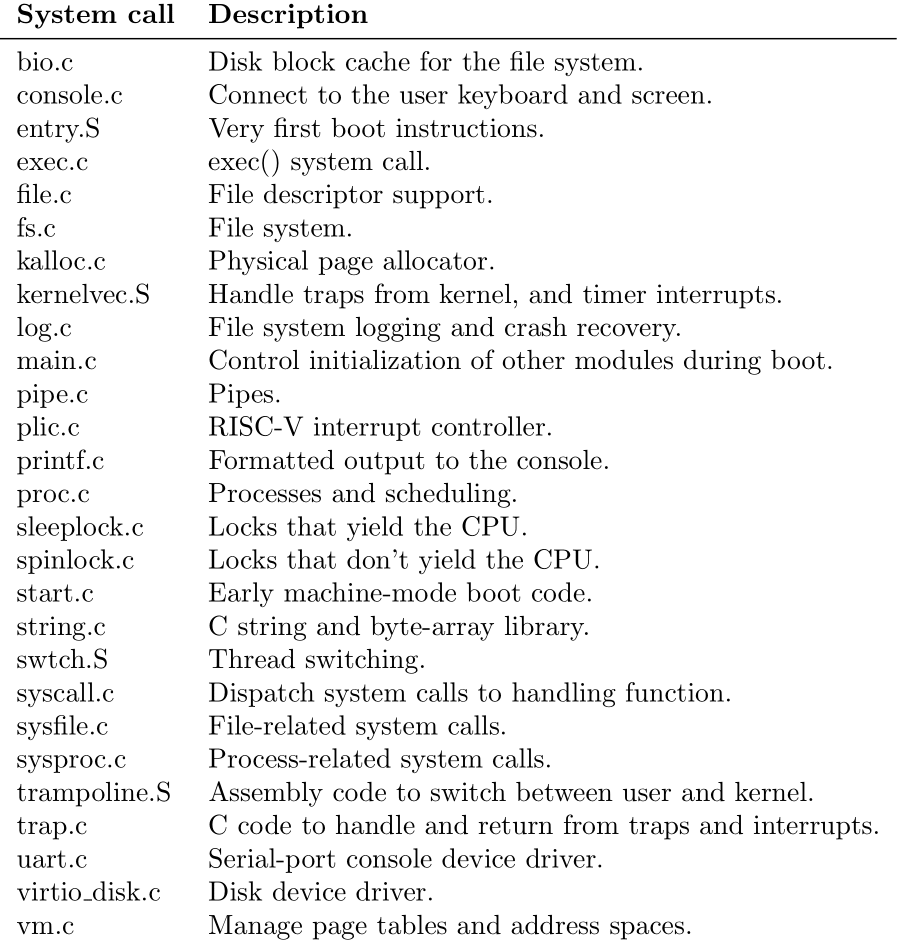
\includegraphics[scale=0.55]{libs/img/estructura_kernel.png}
        \source{xv6: a simple, Unix-like teaching operating system \cite{xv6_book}}
        \label{fig:Estructura_Kernel}
    \end{figure}
\end{frame}
%% ---------------------------------------------------------------------------
\section{Procesos}
\begin{frame}{Procesos}
    La unidad de aislamiento en XV6 es un proceso. Esta abstracción permite tener un mayor control sobre operaciones sobre la memoria, la CPU, los descriptores de archivos, etc. Esto evita que un proceso pueda manipular, espiar o dañar otro proceso o incluso el kernel mismo.

    \vspace{0.3cm}

    El kernel debe tener una implementación segura del proceso, dado que si se presentan errores, estos pueden ser empleados para engañar el kernel o al hardware, siendo una falla de seguridad. Los mecanismos empleados por el kernel para implementar procesos se basan en: indicadores de modo usuario/supervisor, espacios de direcciones y división de tiempo de subprocesos. \cite{xv6_book}
\end{frame}
%% ---------------------------------------------------------------------------
\begin{frame}{Aislamiento}
    Para facilitar el proceso de aislamiento se proporciona la ilusión a un programa de que tiene la totalidad de la máquina para su ejecución. Para lograr la ilusión, al programa se le proporciona un sistema de memoria privada (espacio de direcciones), que no puede ser leída o escrita por algún otro proceso. Adicionalmente, se brinda lo que parece ser su propia CPU para ejecutar las instrucciones del programa.
\end{frame}
%% ---------------------------------------------------------------------------
\begin{frame}
    XV6 implementa un sistema de direcciones basado en tablas de páginas, estas son implementadas por hardware, para administrar un espacio de direcciones virtuales. La tabla de páginas que implementa RISC-V mapea una dirección virtual \emph{(la dirección que manipulan las instrucciones de RISC-V)} a una dirección física \emph{(una dirección que el chip de la CPU envía a la memoria principal)}.\cite{xv6_book}
    \begin{figure}
        \centering
        \caption{Diseño del espacio de direcciones virtuales de un proceso}
        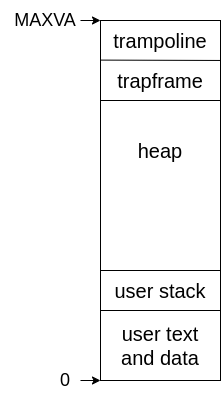
\includegraphics[scale=0.28]{libs/img/as.png}
        \source{xv6: a simple, Unix-like teaching operating system \cite{xv6_book}}
        \label{fig:Espacio_Direcciones}
    \end{figure}
\end{frame}
%% ---------------------------------------------------------------------------
\begin{frame}{Tabla de páginas}
    XV6 brinda una tabla de páginas \emph{para cada proceso}, esta definirá el espacio de direcciones de ese proceso, como se aprecia en la siguiente figura \ref{fig:Espacio_Direcciones}, este espacio de direcciones \emph{incluye la memoria de usuario del proceso}, la cual inicia en la dirección virtual cero. Su estructura en orden creciente de las direcciones es:

    \vspace{0.3cm}
    
    \begin{itemize}
        \item Las instrucciones que ejecutara el proceso
        \item Las variables globales
        \item El stack o pila
        \item El heap o montículo
    \end{itemize}
\end{frame}
%% ---------------------------------------------------------------------------
\begin{frame}{Límites físicos}
    El heap puede ser empleado para expandir el espacio de direcciones según sea necesario, pero este crecimiento está limitado, los punteros en RISC-V tienen un tamaño de 64 bits, pero el hardware, solo usa los \emph{39 bits menos significativos} cuando mapea direcciones virtuales en las tablas de páginas, donde XV6 \emph{solo usa 38 de estos 39 bits}.
    
    \vspace{0.2cm}

    Por lo que \example{la dirección máxima es $2^{38}-1$}, esta se define en la macro \textit{\emph{MAXVA}}, esta se encuentra en \href{https://github.com/CarlosSandoval-03/xv6-riscv/blob/riscv/kernel/riscv.h\#L363}{\textit{\textbf{(kernel/riscv.h:363)}}}. \cite{xv6}
\end{frame}
%% ---------------------------------------------------------------------------
\begin{frame}{Trampolín y Trapframe}
    Hacia las direcciones más altas del espacio de direcciones de memoria, encontramos el espacio de XV6, aquí, se reserva una página para el \textit{\emph{trampoline}} y una página que mapea el \textit{\emph{trapframe}} del proceso. Estas páginas son empleadas por XV6 para hacer la transición entre el kernel y el proceso.

    \vspace{0.3cm}

    Estas páginas se abordarán con más profundidad en próximos capítulos, pero en resumen, la página del trampolín contiene el código para entrar y salir del kernel, mientras el trapframe es usado para almacenar el estado del proceso. \cite{stackoverflow:Trapframe}
\end{frame}
%% ---------------------------------------------------------------------------
\begin{frame}{Estado del proceso}
    El kernel de XV6 almacena en una estructura el estado de cada proceso, esta estructura se define en \href{https://github.com/CarlosSandoval-03/xv6-riscv/blob/riscv/kernel/proc.h\#L85}{\textit{\textbf{(kernel/proc.h:85)}}} \cite{xv6}. Las partes más importantes del núcleo de un proceso son:

    \begin{itemize}
        \item El estado de ejecución \href{https://github.com/CarlosSandoval-03/xv6-riscv/blob/riscv/kernel/proc.h\#L89}{\textit{\textbf{kernel/proc.h:89}}}
        \item La pila del kernel \href{https://github.com/CarlosSandoval-03/xv6-riscv/blob/riscv/kernel/proc.h\#L99}{\textit{\textbf{kernel/proc.h:99}}}
        \item La tabla de páginas \href{https://github.com/CarlosSandoval-03/xv6-riscv/blob/riscv/kernel/proc.h\#L101}{\textit{\textbf{kernel/proc.h:101}}}
    \end{itemize}
\end{frame}
%% ---------------------------------------------------------------------------
\begin{frame}{Hilos}
    Cada proceso tiene un \href{https://en.wikipedia.org/wiki/Thread_(computing)}{\textbf{\textit{hilo o subproceso}}} de ejecución, este es el encargado de ejecutar una serie de instrucciones del proceso, estos hilos pueden ser suspendidos para posteriormente reanudar su ejecución.
    
    \vspace{0.3cm}
    
    Para ejecutar los cambios entre procesos, el kernel \emph{suspende} el hilo que está en ejecución y \emph{reanuda} el hilo relacionado con otro proceso.
    
    \vspace{0.2cm}
    
    El sistema presenta un \href{https://en.wikipedia.org/wiki/Context_switch}{\textit{\textbf{cambio de contexto,}}} a raíz de cambio de estado de un subproceso, para que el sistema lleve a cabo esta operación es necesario que: \example{variables locales, direcciones de retorno de llamadas a funciones}, sean almacenadas en la pila del hilo.
\end{frame}
%% ---------------------------------------------------------------------------
\begin{frame}{}
    Cada proceso tiene dos \href{https://en.wikipedia.org/wiki/Stack-based_memory_allocation}{\textit{\textbf{pilas o stacks}}}: una pila de usuario y una pila del kernel \textit{kstack}.
    
    \begin{itemize}
        \item Cuando el proceso ejecuta instrucciones de usuario, solo emplea la pila de usuario, y su pila de kernel está vacía. 
        \item Cuando el proceso ingresa al kernel (ya sea por una llamada al sistema o una interrupción), el código de manejo, del kernel se ejecutará en la pila del kernel del proceso.
        \item Mientras un proceso este en el kernel, su pila de usuario \emph{aun contiene} datos almacenados, aunque estos no se usen activamente.
    \end{itemize}

    \begin{block}{Pila del kernel}
        La pila del kernel está separada (y protegida del código de usuario), para que el kernel pueda ejecutarse aun cuando un proceso haya estropeado su pila de usuario. \cite{xv6_book}
    \end{block}
\end{frame}
%% ---------------------------------------------------------------------------
\begin{frame}{}
    Un proceso puede realizar una llamada al sistema empleando la instrucción \href{https://jborza.com/emulation/2021/04/22/ecalls-and-syscalls.html}{\textit{\textbf{ecall}}} de RISC-V \cite{xv6_book}. Esta instrucción \emph{eleva} el nivel de privilegio del hardware y \emph{cambia} el \href{https://en.wikipedia.org/wiki/Program_counter}{\textit{\textbf{contador del programa}}} al punto de entrada al kernel definido \cite{xv6_book}.

    \vspace{0.2cm}
    
    El código de manejo, cambia a la pila del kernel y ejecuta las instrucciones para resolver la petición. Cuando finaliza la llamada al sistema, el kernel vuelve a la pila de usuario mediante la instrucción \href{https://jborza.com/post/2021-04-04-riscv-supervisor-mode/}{\textit{\textbf{sret}}}, esta instrucción, reducirá el nivel de privilegio del hardware y reanuda la ejecución de las instrucciones del usuario, justo después de la instrucción de la llamada al sistema \cite{xv6_book}

    \begin{block}{Interrupciones}
        El hilo de un proceso puede ser suspendido por el kernel mientras espera a que se solucione la petición de E/S, y reanudar donde se quedó.
    \end{block}
\end{frame}
%% ---------------------------------------------------------------------------
\begin{frame}{Un vistazo al código}
    En el código fuente de XV6, “p->state” indica si el proceso está asignado, listo para ejecutarse, en ejecución, esperando E/S o finalizando. \cite{xv6_book}

    \vspace{0.3cm}

    Mientras que “p->pagetable”, contiene la tabla de páginas de un proceso, en el formato que maneja el hardware de RISC-V. XV6 se encarga que el hardware de paginación emplee la tabla de páginas de un proceso cuando se ejecuta ese proceso en el espacio de usuario. \example{Esta tabla de páginas actúa como registro de las direcciones físicas de las páginas asignadas a un proceso.} \cite{xv6_book}
\end{frame}
%% ---------------------------------------------------------------------------
\begin{frame}{Resumen}
    Un proceso agrupa unas ideas fundamentales de diseño: un espacio de direcciones para dar al proceso la ilusión de su propia memoria, y un hilo, para dar la ilusión de su propia CPU. \cite{xv6_book}

    \vspace{0.3cm}

    En sistemas operativos más robustos, un proceso puede tener múltiples hilos para aprovechar varias CPU.
\end{frame}
%% ---------------------------------------------------------------------------
\section{Empezando en XV6, el primer proceso y syscall}
\begin{frame}{Arranque}
    Cuando la computadora se enciende, se ejecuta el cargador de arranque almacenado en la memoria \href{https://en.wikipedia.org/wiki/Read-only_memory}{\textit{\textbf{ROM}} (Read-Only Memory)}, el gestor de arranque \emph{carga el kernel de XV6} en la memoria.

    \vspace{0.3cm}

    Cada CPU arranca en modo máquina, el emulador QEMU se encarga de que cada hilo de ejecución del que dispone el hardware vaya al punto de entrada definido en código ensamblador de RISC-V, este punto de entrada se define a través de la etiqueta “\_entry” \href{https://github.com/CarlosSandoval-03/xv6-riscv/blob/riscv/kernel/entry.S\#L7}{\textit{\textbf{kernel/entry.S:7}}}.

    \vspace{0.1cm}

    \begin{block}{Memoria}
        En esta etapa, el hardware de paginación está deshabilitado, por lo que las direcciones virtuales se asignan directamente a las direcciones físicas.
    \end{block}
\end{frame}
%% ---------------------------------------------------------------------------
\begin{frame}{Habilitando la ejecución de código}
    Cuando el kernel es cargado a la memoria, será cargado en la dirección física \textbf{0x80000000}, esta dirección es empleada dado que las direcciones desde \textbf{0x0:0x80000000} son empleados por QEMU para los dispositivos de E/S. \cite{xv6_book} \newline

    \vspace{0.3cm}

    Las instrucciones en \_entry configuran el stack para que XV6 pueda ejecutar código en C. XV6 declara el espacio para la pila inicial, \textbf{stack0}, en el archivo start.c \href{https://github.com/CarlosSandoval-03/xv6-riscv/blob/riscv/kernel/start.c\#L11}{\textit{\textbf{(kernel/start.c:11)}}} \cite{xv6_book}. 
\end{frame}
%% ---------------------------------------------------------------------------
\begin{frame}{}
    El código en \_entry carga la dirección del \textbf{stack+4096} bytes al puntero de pila, esta operación se realiza por cada CPU. En el puntero de la pila se carga la dirección más alta, dado que en RISC-V \emph{la pila crece hacia direcciones más bajas}.\newline
    
    \vspace{0.3cm}
    
    Una vez está asignado la pila del kernel, \_entry ejecuta la función de inicio \href{https://github.com/CarlosSandoval-03/xv6-riscv/blob/riscv/kernel/start.c\#L21}{\textbf{\textit{(kernel/start.c:21)}}}. \cite{xv6_book}
\end{frame}
%% ---------------------------------------------------------------------------
\begin{frame}{Configurando el sistema}
    Después de ser invocada por \_entry, la función de inicio se encarga de realizar las configuraciones para iniciar el sistema, algunas de estas operaciones solo se permiten en el modo máquina, después de finalizar las operaciones que lo requieren, XV6 reducirá su privilegio sobre el hardware, al modo supervisor. 

    \vspace{0.4cm}

    RISC-V proporciona la instrucción “mret”, esta instrucción se suele emplear para regresar a un nivel de privilegios anterior, por ejemplo: si ocurre una excepción en el modo supervisor, la CPU cambiará al modo máquina para ejecutar las directrices de manejo de la excepción, una vez finalice este proceso, se empleará mret para retornar al modo supervisor.
\end{frame}
%% ---------------------------------------------------------------------------
\begin{frame}{Configuraciones en modo máquina}
    Respecto al manejo de mret, se presenta un problema, la función start no regresa de una llamada de este tipo, por lo que se configura el sistema como si lo hiciera, estas configuraciones son:

    \vspace{0.3cm}

    \begin{itemize}
        \item Se define el “modo anterior”, a modo supervisor, esto mediante el cambio en el registro \textbf{mstatus}.
        \item Establece la \emph{dirección de retorno en el método main}, escribiendo la dirección de dicho método en el registro \textbf{mepc}.
        \item  Deshabilita la paginación en modo supervisor, esto se realiza escribiendo un 0 en el registro \textbf{satp} de la tabla de páginas.
        \item Delega todas las interrupciones y excepciones al modo supervisor.
    \end{itemize}
\end{frame}
%% ---------------------------------------------------------------------------
\begin{frame}{}
    Continuando con las operaciones de configuración:
    \begin{itemize}
        \item Concede al modo supervisor el acceso \emph{toda} la memoria física, mediante la configuración de la protección de memoria física.
        \item Programa el chip del reloj para recibir interrupciones del temporizador.
        \item Almacena el identificador de cada CPU en el registro de hilo \textbf{(thread pointer o tp)}
    \end{itemize}

    \vspace{0.3cm}

    Una vez se finaliza esta configuración, se ejecuta la instrucción de retorno, esto para “regresar” al modo supervisor y cambiando el puntero del programa \textbf{(stack pointer o sp)} a la función main, esta función se define en \href{https://github.com/CarlosSandoval-03/xv6-riscv/blob/riscv/kernel/main.c\#L11}{\textbf{\textit{(kernel/main.c:11)}}}. \cite{xv6_book} \cite{xv6}
\end{frame}
%% ---------------------------------------------------------------------------
\begin{frame}{Iniciando el sistema}
    La función main, primero reconoce la CPU con ID 0, y este se encargará de inicializar y configurar diversos sistemas, algunas de las tareas que realiza son:

    \vspace{0.2cm}
    
    \begin{itemize}
        \item Inicia la consola.
        \item Habilita la salida estándar (printf).
        \item Inicia el asignador de páginas físicas.
        \item Crea la tabla de páginas del kernel.
        \item Habilita la paginación.
        \item Inicia la tabla de procesos
    \end{itemize}
    
    \vspace{0.2cm}

    Entre otras muchas configuraciones, pero el primer proceso de usuario que ejecuta es userinit, el cual se define en \href{https://github.com/CarlosSandoval-03/xv6-riscv/blob/riscv/kernel/proc.c\#L233}{\textbf{\textit{kernel/proc.c:233}}} \cite{xv6}.
\end{frame}
%% ---------------------------------------------------------------------------
\begin{frame}{Primer proceso de usuario}
    El primer proceso de usuario ejecuta un código ensamblador, este está definido en \href{https://github.com/CarlosSandoval-03/xv6-riscv/blob/riscv/user/initcode.S}{\textbf{\textit{user/initcode.S}}}, este código prepara el uso de la syscall \textbf{exec}.
    
    \vspace{0.3cm}

    Primero, carga la dirección del método \textbf{init} en el registro \textbf{a0}, luego la dirección del arreglo con los argumentos de la llamada \textbf({argv)} al registro \textbf{a1}, despues carga el número que identifica la llamada al sistema de \href{https://github.com/CarlosSandoval-03/xv6-riscv/blob/riscv/kernel/syscall.h\#L8}{SYS\_exec \textbf{\textit{(kernel/syscall.h:8)}}} en el registro \textbf{a7}, y finalmente llama a ecall para ingresar de nuevo al kernel. \cite{xv6_book}
\end{frame}
%% ---------------------------------------------------------------------------
\begin{frame}{Preparando el espacio de usuario}
    El kernel emplea el número de la llamada al sistema almacenada en el registro a7 para ejecutar la llamada indicada \href{https://github.com/CarlosSandoval-03/xv6-riscv/blob/riscv/kernel/syscall.c\#L132}{\textbf{\textit{(kernel/syscall.c:132)}}}. Estos identificadores son asignados en \href{https://github.com/CarlosSandoval-03/xv6-riscv/blob/riscv/kernel/syscall.c\#L107}{\textbf{\textit{kernel/syscall.c:107}}}, donde se relaciona a la constante SYS\_exec con el método sys\_exec, que invoca el kernel. \cite{xv6_book}

    \vspace{0.3cm}

    Como se trató en el capítulo 1, exec reemplaza la memoria y los registros del proceso actual con una nueva imagen ejecutable \emph{(en este caso /init)}.
\end{frame}
%% ---------------------------------------------------------------------------
\begin{frame}{Iniciando el espacio de usuario}
    Una vez el kernel finaliza estas operaciones, “regresa” al espacio del usuario en el proceso init \href{https://github.com/CarlosSandoval-03/xv6-riscv/blob/riscv/user/init.c\#L15}{\textbf{\textit{(user/init.c:15)}}}. Este proceso inicia la consola, si es necesario crea un nuevo archivo de dispositivo que referencia la consola, luego lo abre como descriptores de archivo con los valores estándar (0, 1 y 2). Inicia un Shell en la consola.

    \vspace{0.2cm}

    \emph{El sistema está activo!!!}
\end{frame}
%% ---------------------------------------------------------------------------
\section{Modelo de seguridad}
\begin{frame}{Seguridad en el sistema operativo}
    El enfoque respecto al diseño que se debe implementar es, asumir que \emph{todo} código de nivel de usuario de un proceso buscara de \emph{todas las formas posibles} arruinar el kernel u otros procesos.

    \vspace{0.3cm}

    \begin{itemize}
        \item Referenciar puntos fuera de su espacio de direcciones permitido.
        \item Ejecutar instrucciones de la CPU aunque estas no estén permitidas al usuario.
        \item Intentar leer o escribir sobre registros de control de RISC-V.
        \item Intentar acceder directamente al hardware del dispositivo.
        \item Pasar argumentos a las llamadas al sistema que busquen entorpecer o bloquear el kernel.
    \end{itemize}
\end{frame}
%% ---------------------------------------------------------------------------
\begin{frame}{}
    El objetivo del kernel es restringir los procesos de cada usuario para que solo pueda leer/escribir/ejecutar su espacio de direcciones asignado, emplear los 32 registros de RISC-V de propósito general, emplear llamadas al sistema que modifiquen otros proceso o el kernel de manera segura. Es un requisito absoluto que el \emph{kernel evite cualquier otra acción que el usuario desee ejecutar}. \cite{xv6_book}
\end{frame}
%% ---------------------------------------------------------------------------
\begin{frame}{Comunidad y enfoque}
    Se asume que el código del kernel está escrito por programadores cuidadosos y sin malas intenciones, se espera que el código del kernel este libre de errores y no contenga nada malicioso. \cite{xv6_book} \newline
    \example{Algunas funciones como el spinlock puede generar múltiples problemas si se usa de manera incorrecta}

    \vspace{0.3cm}

    Esto debe estar presente al momento de leer el código, se debe suponer que el código está escrito correctamente, también que este sigue todas las reglas sobre el uso de funciones y estructuras de datos propias del kernel \cite{xv6_book}. Igualmente, se supone que el hardware funciona como se define en la documentación, y que no se presentan errores.
\end{frame}
%% ---------------------------------------------------------------------------
\begin{frame}{}
    Claramente, estos son escenarios idealistas, no es tan simple evitar que el código ejecutado en espacio de usuario ocasione que el sistema quede inutilizable o que esté entre en pánico, principalmente porque el código malicioso intenta consumir recursos protegidos por el kernel, como: espacio en disco, tiempo de CPU, entradas de la tabla de procesos, etc. \cite{xv6_book}

    \vspace{0.3cm}

    Generalmente, es imposible escribir código sin errores o diseñar de hardware libre de errores, por lo que si desarrolladores maliciosos están al tanto de los errores del kernel o el hardware, los explotarán. \cite{xv6_book}
\end{frame}
%% ---------------------------------------------------------------------------
\begin{frame}{}
    Incluso en kernels maduros y de alto uso, como Linux, se descubren nuevas vulnerabilidades continuamente; por lo que, vale la pena diseñar sistemas de protección en caso de que el kernel contenga errores, algunas de las estrategias de protección son:

    \begin{itemize}
        \item \href{https://en.wikipedia.org/wiki/Assertion\_(software\_development)}{\textbf{\textit{Aserciones}}}
        \item Verificación de tipos
        \item Páginas de protección de la pila
        \item Entre otros
    \end{itemize}
\end{frame}
%% ---------------------------------------------------------------------------
\section{Mundo real}
\begin{frame}{Mundo real}
    La distinción entre el código del usuario y del kernel suele ser distorsionada. Algunos procesos de nivel de usuario pueden brindar servicios esenciales y ser parte del sistema operativo de manera efectiva, y en algunos sistemas operativos, el código de usuario puede insertar nuevo código en el kernel (como con los módulos del kernel de Linux). \cite{xv6_book}
\end{frame}
%% ---------------------------------------------------------------------------
\begin{frame}{Implementaciones modernas}
    La mayoría de los sistemas operativos modernos emplean el concepto de proceso, siendo similares a la implementación de XV6; sin embargo, los sistemas modernos brindan soporte de subprocesos dentro de un proceso, esto permite que un solo proceso emplee varias CPU. \newline
    \emph{XV6 no proporciona el soporte para múltiples subprocesos.}
\end{frame}

% \section{Tablas de páginas}
% \section{Hardware de paginación}
% \section{Espacio de direcciones del kernel}
% \section{Código: Creando un espacio de direcciones}
% \section{Asignación de memoria física}
% \section{Código: Asignador de memoria física}
% \section{Espacio de direcciones de un proceso}
% \section{Código: sbrk}
% \section{Código: exec}
% \section{Mundo real}

    % \begin{figure}
        % \centering
    %     \caption{Diseño del espacio de direcciones virtuales de un proceso}
    %     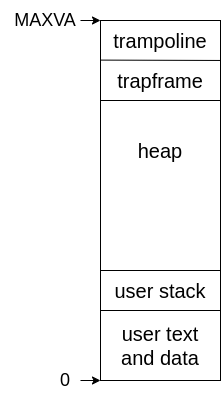
\includegraphics[scale=0.3]{libs/img/as.png}
    %     \source{xv6: a simple, Unix-like teaching operating system \cite{xv6_book}}
    %     \label{fig:Espacio_Direcciones}
    % \end{figure}

% %% ---------------------------------------------------------------------------
% \subsection{subsección 2}
% \begin{frame}{Bloques}
%     % Blocks styles
%     \begin{block}{Bloque azul}
%         fondo bloque en blanco.
%     \end{block}

%     \begin{alertblock}{Bloque de alerta}
%         fondo bloque en blanco.
%     \end{alertblock}

%     \begin{exampleblock}{Bloque de ejemplo}
%         fondo bloque en blanco..
%     \end{exampleblock}   
% \end{frame}

% %% ---------------------------------------------------------------------------
% \subsection{uso de cajas con enfasis}
% \begin{frame}{Para el uso con cajas, en especial programación}
%     \successbox{cajas de test}

%     \pause

%     \alertbox{Alerta de test}

%     \pause

%     \simplebox{Estado de test}
% \end{frame}

% %% ---------------------------------------------------------------------------
% \subsection{Algoritmos}
% \begin{frame}{para Algoritmos (Pseudocódigo)}
%     \begin{algorithm}[H]
%         \SetAlgoLined
%         \LinesNumbered
%         \SetKwInOut{Input}{input}
%         \SetKwInOut{Output}{output}
%         \Input{x: float, y: float}
%         \Output{r: float}
%         \While{True}{
%           r = x + y\;
%           \eIf{r >= 30}{
%            ``O valor de $r$ é maior ou iqual a 10.''\;
%            break\;
%            }{
%            ``O valor de $r$ = '', r\;
%           }
%          } 
%          \caption{Algorithm Example}
%     \end{algorithm}
% \end{frame}

% %% ---------------------------------------------------------------------------

% \begin{frame}{Insertando Algoritmos}
%     \lstset{language=Python}
%     \lstinputlisting[language=Python]{code/main.py}
% \end{frame}

% %% ---------------------------------------------------------------------------
% \begin{frame}{Insertando Algoritmos}
%     \lstinputlisting[language=C]{code/source.c}
% \end{frame}

% %% ---------------------------------------------------------------------------
% \begin{frame}{Insertando Algoritmos}
%     \lstinputlisting[language=Java]{code/helloworld.java}
% \end{frame}

% %% ---------------------------------------------------------------------------
% \begin{frame}{Insertando Algoritmos}
%     \lstinputlisting[language=HTML]{code/index.html}
% \end{frame}

% %% ---------------------------------------------------------------------------
% % This frame show an example to insert multicolumns
% \section{Sección II}
% \begin{frame}{Sección II}
%     \begin{columns}{}
%         \begin{column}{0.5\textwidth}
%             \justify
%            utilizado y justificado para 2 columnas
%         \end{column}
%         \begin{column}{0.5\textwidth}
%             \justify
%            espacioentre columnas para un segundo argumento
%         \end{column}
%     \end{columns}    
% \end{frame}

% %% ---------------------------------------------------------------------------
% % This frame show an example to insert figures
% \section{sección III}
% \begin{frame}{Sección III - Figuras}
%     \begin{figure}
%         \centering
%         \caption{logo UNAL.}
%         
\includegraphics[scale=0.3]{libs/UNAL_logo.jpg}
%         \source{Obtenido del sitio oficial \cite{xv6} \cite{xv6_book}}
%         \label{fig:Logo UNAL}
%     \end{figure}
% \end{frame}

%% ---------------------------------------------------------------------------
% Reference frames
\begin{frame}[allowframebreaks]
    \frametitle{Referencias}
    \printbibliography
\end{frame}

%% ---------------------------------------------------------------------------
% Final frame
\begin{frame}
    \centering
    \huge{\textbf{\example{Gracias por la atención}}}
    
    \vspace{1cm}
    
    \Large{\textbf{Contacto:}}
    \newline
    \vspace*{0.5cm}
    \large{\email{csandovalc@unal.edu.co}}
\end{frame}

\end{document}